% results.tex -- \section{Results} for the ICLR 2027 main file.
% Written 2026-09-12 against the corrected record; audit fixes applied 2026-09-12;
% revised 2026-09-12 (evening) for the 16.10, 16.14b and 16.15 RESULTS blocks per
% papers/embodied_sensor/AUDIT_16_15_consequences.md. Every number carries a LaTeX
% comment naming its source line. Abbreviations in comments:
%   prereg = Guidance_Documents/prereg_embodiment_community.md; only lines inside a
%            RESULTS block are cited for findings (E1 RESULTS L139-330, E2/E3 L331-393,
%            E5 L526-579, L1 L580-676, L2 L677-851, ACTUATOR LADDER L852-984, Dilemmas
%            Stage 1 L2406-2564, Stage 2 L2565-2715, 13.1 L2716-3032, 16.8 L3377-3503,
%            16.11a L3608-3638, 16.11b L3639-3654, 16.14b L4091-4134, 16.10 L4136-4210,
%            16.15 L4212-4717, 16.13 Stage A and B1 L4719-4791, 16.12 RESULTS note
%            L4992-5016, 16.13 Stage B2 L5018-5058, 16.13c Stage C1 L5060-5106, 16.13d
%            L5147-5192; the 16.13c amendment L4961-4990 and the 16.13d registration
%            L5108-5145 are cited for definitions only). The Addendum 16.12 table
%            (L3655-3703) sits under a non-RESULTS heading; its cells are now reproduced
%            in the 16.12 RESULTS note (L4992-5016) with the artefact
%            flooding_analysis.json, and the flooding paragraph still reads the 16.15.1
%            RESULTS block and router_decomposition.json.
%   JSON   = divergence_study_outputs/<file> unless another path is given
% Style matches introduction.tex: no em dashes, no colons or semicolons in running
% prose, no lists, past tense for what was done, present for what holds.
% Terminology as introduction.tex: embodiment assigns a perspective and at full dose
% an interest; narration is the light dose, advocacy the full dose; the collective is
% the three-seat graph; "the sensor" is the flag that fires when the second advocate
% objects (the stake-blind counter, two or more seats objecting); "one effective
% voter" always carries its scope clause (where the roles lock).
% Bib key used here exists in references.bib: cheng25elephant (petrov2025brokenmath is
% cited in methods.tex, the BrokenMath clause having left this file's opening for budget).
% No bib key exists for the Scruples corpus, so it is not cited by key.
%
% CHANGES IN THIS REVISION, for the PI:
%  (a) Contribution 1 gains the 16.14b cycling result, the 16.15.5 committed-only /
%      Manski sentence and the 16.15.7 intervals on the four manner drops; the
%      role-lock paragraph moves here as the advocacy dose, matching the
%      introduction's first contribution (embodiment as a control).
%  (b) Contribution 2 is the one-effective-voter result with its registered readout
%      (1,642 of 1,642; CV oracle gap +0.000 [-0.004, +0.000]) and the 16.10 two-by-two
%      as centrepiece (new Table tab-topology). The record's "1,663 of 1,663" and the
%      full-profile oracle gap -0.021 are dropped (no r0-cache population reproduces
%      1,663; -0.021 carries no interval and is not computable within 16.15.4).
%  (c) Contribution 3 is rewritten around 16.15.1-16.15.3. The transfer rows and
%      Figure 3 now use the stake-blind counter throughout (the introduction's
%      sensor), from transfer_readouts.json.
%  (d) DROPPED for lack of a RESULTS line or JSON artefact (house rule): the pooled
%      writer-counterparty phi -0.719 and the two neutral-edge phis (html L46 / 16.8
%      preamble only); the +0.069 [+0.043, +0.097] and +0.053 [+0.029, +0.079]
%      solo-minus-collective contrasts (html L44 only); the +0.014 [+0.000, +0.028]
%      neutral-opening-minus-protocol contrast (html L44 only); the cross-model
%      counter lifts +0.133 / +0.039 and fire rates 0.161 / 0.762 for haiku / nano
%      (prereg L3144-3147, Addendum 16.4, a non-RESULTS heading, no JSON), with which
%      Figure 2 (fig-grip) and the "tracks grip, not accuracy" sentence go. Each can
%      be restored by a zero-spend artefact.
%  (e) FIGURES REGENERATED 2026-09-12 (make_figures.py, zero spend, JSON only):
%      fig3 reads transfer_readouts.json targets.*.by_sensor.counter and
%      router_decomposition.json counter_lift_by_stratum.pooled; fig4 lost its phi
%      panel (no artefact at the time; flooding_analysis.json now carries the per-type
%      phis, see (f)) and its accuracy panel reads effective_voter.json panels.grok,
%      router_decomposition.json composed_haiku.routers.collective_alone and
%      transfer_readouts.json targets.grok_solo_standard; fig5 reads
%      router_decomposition.json composed_haiku (counter, verdict type, union, random at
%      the union's coverage) with haiku everywhere 0.850 from prereg L891. fig2 is not
%      referenced and is not regenerated from any source the paper cites.
%  (f) The phi artefact now exists: prereg L4992-5016 (16.12 RESULTS note, zero spend)
%      and flooding_analysis.json aita.populations.s2_codable_16_12.groups.{YTA,NTA,ESH,
%      NAH,one_loser,both_party,pooled}.phi_advocates (YTA -0.340 [-0.663, +0.011], NTA
%      -0.162 [-0.317, -0.022], ESH -0.191 [-0.265, -0.112], NAH -0.275 [-0.564, +0.009],
%      pooled one-loser -0.901 [-0.929, -0.868]); the record cautions (L5002-5007) that
%      the pooled one-loser phi is carried by which seat loses and the within-type phi
%      is weak. Not restored to the prose or to fig4 for budget; if restored, plot the
%      per-type phis with intervals and carry the L5002-5007 caution in the caption.
%      Still pending as zero-spend notes:
%      rolelock_by_model.json and length_matched_elephant_oeq_validation_corrected.json
%      to be appended to the prereg as dated zero-spend notes; role-lock 0.9712
%      (rolelock_by_model.json, effective_voter.json) against 0.9717 at the 16.8
%      preamble L3277, PI to reconcile.
%  (g) The 16.13 RESULTS blocks (Stage A and B1, Stage B2, 16.13c Stage C1 and 16.13d)
%      are reported in sec-results-extent as a measured boundary of the theory.
%  (h) Zero-spend audit pass 2026-09-12 (later): B2 role-lock restated over all 144
%      games; mediator Nash-pull 20 of 21, not every game; 98.75 and 95 percent levels
%      separated in the routing paragraph; the sonnet routing of the model's own
%      disagreement alone noted as absent from the record; D2 rested on the neutral arm
%      with the planner arm's seed-dependent lower bound stated; the coordination gain
%      qualified by the scoring rule and the eleven equilibrium recommendations; what the
%      roles contributed on the games stated with the record's non-separability; the
%      "independent nodes" clause corrected for the moderator hub; comment line ranges
%      corrected to the 5,192-line record; prose cut to budget.

\providecommand{\todo}[1]{\textbf{[TODO: #1]}}

\section{Results}
\label{sec-results}

Five instruments carry the results (Table~\ref{tab-instruments}).
% The 249 conflict accounts, 99 gold at-fault and 150 not (crowdgold_aita_summary.json:7-11),
% the 210 the collective deliberated after the content filter (prereg L528-531, L534-537,
% E5 RESULTS) and the 100 false-premise statements from BrokenMath (prereg L42-48 design,
% L139 E1 RESULTS heading) are described and cited in methods.tex sec-method-instruments and
% tab-instruments; the clauses were dropped here for budget. Figure fig-rolelock marks the
% gold base rate.
% Open-ended accounts (150 per generator, length_matched_elephant_oeq_validation_corrected_16_15_7.json:6-11)
% enter only in sec-results-control, and the paired-account Dilemmas and the 144 games
% (methods.tex tab-instruments, games row) only in sec-results-extent.
Intervals are 95 percent item-clustered bootstraps unless another level is
named. % prereg L75-76 (10,000 draws, false premise); L4226-4228 (16.15, 4,000 draws seed 13); stake_grip_analysis.json (2,000, grip)
% Crowd verdicts are scored by the registered five-token collapse, prereg L3395-3399
% (16.8 RESULTS, the applied convention), L4230 (16.15); stated in methods.tex.

\subsection{Embodiment places the bias}
\label{sec-results-control}

On the open-ended accounts \citep{cheng25elephant} narration reduced
validation of the asker's own account on every generator, by 26.7 points
[16.7, 36.7] on haiku, 22.3 [13.3, 31.3] on sonnet, 41.4 [31.4, 51.1] on
nano and 36.0 [27.1, 44.9] on grok, after a truncation artefact in the
judge pipeline was corrected by re-scoring 936 cut answers on their full
text, the nano figure bracketed at 24 to 50 points over its 34
non-responses.
% prereg L4595-4600 (16.15.7 RESULTS, "replaced 936 truncated scores", "the four drops are
% fully corrected"); bm_notes.json 16.15.7 corrected_line.replaced 936. Drops from prereg
% L4609-4612 (16.15.7 RESULTS table, drop (pp) [95% CI]); bm_notes.json 16.15.7
% drops.*.delta_pp and ci_pp (8,000 draws, seed 20260822); rates 0.627/0.360,
% 0.727/0.503, 0.759/0.345, 0.815/0.455 in the same rows. The uncorrected deltas in
% elephant_summary.json (-36.0 / -25.7 / -48.4 / -52.5) must NOT be used.
% Nano CoT n / NoT n 145 / 116 (116 of 150 narrated responses scored), Manski bracket
% [-50.000, -24.000], prereg L4611; bm_notes.json 16.15.7 drops.gpt-5.4-nano.manski_bracket_pp,
% nonresponse_not.missing 34.
% Grok's bracket is 32 to 38 (L4612), dropped for budget.
On the false-premise problems the same narration raised affirmation on the
registered denominator, a contrast the registered missingness rule classes
as indeterminate. The untreated model affirmed the false premise at 0.157
and under narration at 0.223, % prereg L166-167 (E1 RESULTS)
the registered contrast was +0.067 [+0.033, +0.103], % prereg L4534-4536 (16.15.5 RESULTS); bm_embody_analysis.json:124-129
% The replicate gap of +0.010 [-0.013, +0.033] between two untreated arms,
% bm_embody_analysis.json:130-135 (S0_replicate_gap_standard_minus_duplicate; :44-48 the
% 0.147 one-line baseline), was dropped from the prose for budget; it is artefact-only.
% Prereg L23-31 is the pre-RESULTS "Instrument note discovered during design", cited only
% as design context for why the one-line arm is a standard_cot replicate, not as a source
% of the value. The 0.157 is the registered E1 value; the live cache reads 0.172 after a
% later backfill of sixteen records, prereg L4681-4687.
the committed-only contrast, with the 34.5 and 27.8 percent of the 600 units
per arm that returned no verdict removed, was +0.070 [+0.030, +0.115], and
the Manski bounds on the registered contrast, [-0.278, +0.345], cross zero.
% prereg L4533-4541, L4546-4547, L4557-4559 (16.15.5 RESULTS, the three readouts in one
% sentence as the pre-declared reading requires); bm_notes.json 16.15.5 arms.*.missing_rate
% and committed_only, snapshot.committed_only.contrast, manski_S0_contrast; rule prereg L105-107.
% The committed-only rates 0.239 [0.153, 0.329] to 0.309 [0.222, 0.398] (same lines) dropped
% for budget.

Assigning an interest without narration moved commitment far less. As the
statement's author the model affirmed it at 0.192 and as the author's rival
at 0.163, % prereg L150-151 (E1 RESULTS; denominators 600 planned units)
a contrast of +0.028 [+0.000, +0.058]. % prereg L154; bm_embody_analysis.json:50-55; every interest arm sat inside [0.157, 0.192] (colleague 0.157, stranger 0.180 at L150-151) while narration alone stood at 0.223 (L166-167), dropped for budget
Combining the two did not add, a difference in differences of -0.025
[-0.070, +0.022]. % prereg L348-352 (E2 RESULTS, arms converge to 0.228 / 0.240 / 0.228); bm_cross_sig_analysis.json:37-41; penalty by role L357-360
The reversal is also a first-pass effect, repeated narration eroding the
perspective rather than deepening it. % prereg L4115-4122 (16.14b reading)
% Narration and interest were substitutes, not complements (prereg L348-352), dropped for budget.
Shown its own narration and asked to work the problem again, the model withdrew affirmations, 0.300 to 0.224 on
434 matched units, -0.076 [-0.104, -0.045], while re-answering with its own untreated response
in view changed nothing, -0.003 [-0.025, +0.020], a difference in
differences of -0.073 [-0.107, -0.039].
% prereg L4102-4104, L4106-4108, L4129-4131 (16.14b RESULTS, GUARD OK, primary READ);
% bm_cycleb_analysis.json arms.narrative_cot.p_true / narrative_cot_cycle2b.p_true,
% flip_true_to_false 33, flip_false_to_true 5 (33 flips from TRUE to FALSE against 5 the
% other way, dropped from the prose for budget), contrasts (4,000 draws, seed 11).
% The 16.14 depth-2 block at L3817-3870 is GUARD FLAGGED and is not tabulated.

Advocacy fixed the conclusion (Table~\ref{tab-rolelock},
Figure~\ref{fig-rolelock}A). On grok the writer's advocate found the writer
at fault on 0.3 percent of its opening statements and the other party's
advocate on 97.4 percent, a role-lock of 0.971 [0.954, 0.986] on 1,666
debates, while the seat with no interest sat at 0.430.
% rolelock_by_model.json grok (p_at_fault 0.0030 / 0.9742 / 0.4299, n_r0 1666, role_lock
% 0.9712); interval effective_voter.json panels.grok.role_lock; prereg L3404-3405 (16.8
% RESULTS), L4496 (16.15.4 RESULTS)
Lock is graded across models (Table~\ref{tab-rolelock}),
% rolelock_by_model.json sonnet 0.677 / nano 0.620 / haiku 0.442 role_lock; prereg L4497-4499
and removing the stake clause while keeping the directional assignment left
grok's seats at 0.946 on 377 debates, % prereg L3377, L3404-3405, L3421-3422 (16.8 RESULTS)
so the pinning force was the assignment, not the stake.

\begin{table}[t]
\centering
\caption{Role-lock and seat accuracy at the opening statement by model of the
collective. Lock is $|P(\text{at-fault})_{\text{writer}} -
P(\text{at-fault})_{\text{counterparty}}|$. The stake-removed row keeps the
directional assignment without the stake clause, and its seat accuracies were
not computed. Seat accuracies are on each seat's codable opening verdicts
(1,666, 1,665 and 1,670 on grok), and the prose uses the 1,642 debates where
all three are codable, so 0.857 here and 0.860 there are one quantity on two
denominators.}
% rolelock_by_model.json grok n_codable_by_seat (writer 1666, counterparty 1665, neutral
% 1670) and seat_acc (0.592 / 0.437 / 0.857); effective_voter.json panels.grok
% seat_acc_on_triples (0.591 / 0.437 / 0.860 on n_triples 1642); prereg L4496, L4676-4679
\label{tab-rolelock}
\footnotesize
\setlength{\tabcolsep}{3pt}
\begin{tabular}{lrcccrccc}
\toprule
 & & \multicolumn{3}{c}{$P(\text{at-fault})$ at opening} & & \multicolumn{3}{c}{seat accuracy} \\
\cmidrule(lr){3-5} \cmidrule(lr){7-9}
model & $n$ & writer & counterparty & neutral & lock & writer & counterparty & neutral \\
\midrule
grok        & 1,666 & 0.003 & 0.974 & 0.430 & 0.971 & 0.592 & 0.437 & 0.857 \\ % rolelock_by_model.json grok; prereg L3404-3405 (16.8 RESULTS)
grok, stake removed & 377 & 0.008 & 0.954 & 0.387 & 0.946 & n/a & n/a & n/a \\ % prereg L3377, L3404-3405, L3421-3422 (16.8 RESULTS)
sonnet      & 31    & 0.258 & 0.935 & 0.452 & 0.677 & 0.806 & 0.516 & 1.000 \\ % rolelock_by_model.json sonnet (tag cg_deliberation_sonnet_fixed)
nano        & 816   & 0.147 & 0.767 & 0.363 & 0.620 & 0.718 & 0.612 & 0.830 \\ % rolelock_by_model.json nano (tag cg_deliberation_nano)
haiku       & 190   & 0.474 & 0.915 & 0.656 & 0.442 & 0.816 & 0.444 & 0.708 \\ % rolelock_by_model.json haiku (tag cg_deliberation_haiku_fixed); per-seat codable denominators, see prereg L4676-4679
\bottomrule
\end{tabular}
\end{table}

\begin{figure}[t]
\centering
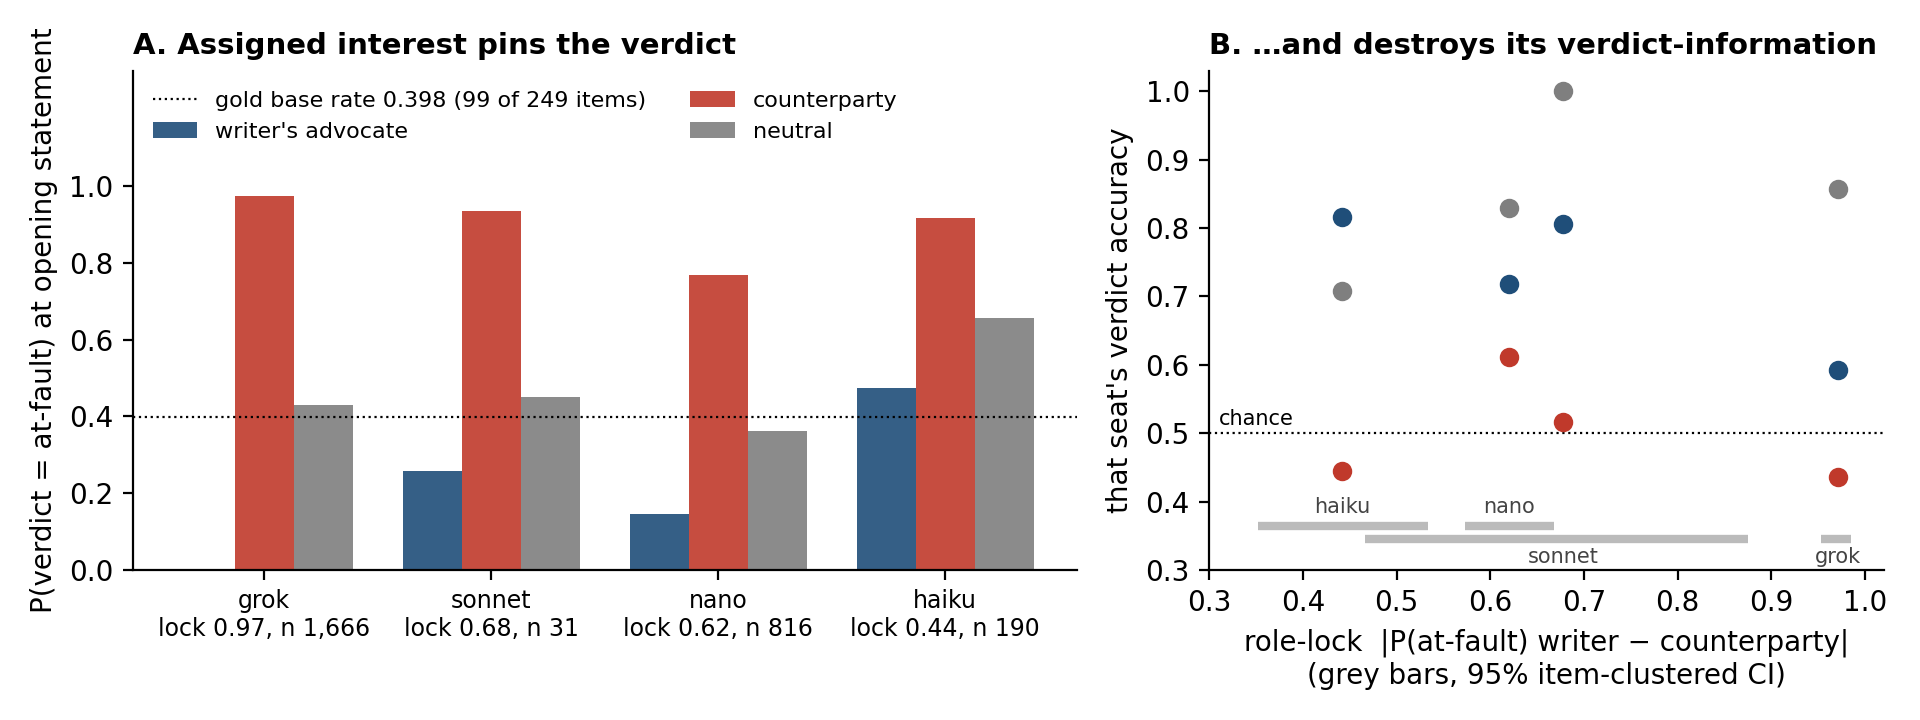
\includegraphics[width=\linewidth]{figures/fig1.png}
\caption{Advocacy as control, and its cost. (A) Probability that each seat's
opening verdict is at-fault, four models, with the gold base rate marked.
(B) Each seat's verdict accuracy against its model's role-lock. The writer's
advocate scores 0.816 at the lowest lock and 0.592 at the highest.}
% make_figures.py Fig 1, read from divergence_study_outputs/rolelock_by_model.json
\label{fig-rolelock}
\end{figure}

\subsection{The collective has one effective voter where the roles lock}
\label{sec-results-collective}

A locked seat carried almost nothing about the case, the two advocates
scoring 0.591 and 0.437 against the crowd on grok while the neutral seat
scored 0.860, on the 1,642 debates with three codable opening verdicts
(Figure~\ref{fig-rolelock}B).
% effective_voter.json panels.grok.seat_acc_on_triples (0.5914 / 0.4373 / 0.8599); prereg
% L4496 (16.15.4 RESULTS). One denominator in prose; Table tab-rolelock and Figure
% fig-rolelock carry the per-seat codable values (0.592 / 0.437 / 0.857 on 1,666,
% rolelock_by_model.json). The 0.816 at the lowest lock (haiku) is in the caption. The
% four-model ordering is not monotone (0.816 / 0.718 / 0.806 / 0.592 by ascending lock,
% sonnet on n=31), so only the extremes are claimed.
So where the roles locked the collective had one effective voter
(Figure~\ref{fig-localisation}B), the three-seat majority equalling the
neutral seat's verdict on 1,642 of those 1,642 debates and the
cross-validated best fixed function of the three opening verdicts being
the neutral seat's own, a gap of +0.000 [-0.004, +0.000] against its
0.860 [0.822, 0.896].
% prereg L4462-4475, L4496, L4506-4510 (16.15.4 RESULTS); effective_voter.json panels.grok
% (210 items) majority_equals_neutral (1642 of 1642), cv_oracle_bits (gap 0.0 [-0.0042, 0.0]),
% seat_acc_on_triples.neutral_adjudicator (0.8599 [0.8223, 0.8965]); 4,000 draws, seed 13
The count holds only where lock does. On nano at lock 0.620 the majority
equalled the neutral seat on 777 of 781 debates, and on haiku at lock 0.442
the writer's advocate outscored the neutral seat, 0.818 against 0.717 on
187 debates, +0.102 [+0.028, +0.182], the majority still tracking it on
180 of 187, so haiku is the boundary of the claim.
% prereg L4498-4499, L4516-4525 (16.15.4 RESULTS); effective_voter.json panels.nano
% majority_equals_neutral 777/781, role_lock 0.6204; panels.haiku role_lock 0.4417,
% seat_acc_on_triples writer 0.8182 / neutral 0.7166, writer_minus_neutral 0.1016
% [0.0276, 0.1818], majority_equals_neutral 180/187. Sonnet (31 debates, 16 items) is
% not a scope datum, prereg L4525-4528.

The two-by-two of roles and edges (Table~\ref{tab-topology}, Figure~\ref{fig-topology}) says which
creates the structure. With the edges cut, role-lock, the localisation
excess and the stake concentration G3 held, and with three identical
readers on the same protocol they vanished, the registered reading H-ROLE,
the structure coming from directional role assignment.
% prereg L4146-4150, L4171-4174 (16.10 RESULTS); topology_2x2_analysis.json cells.*.role_lock,
% objection.localisation_excess, g3.delta; the values (0.969, +0.318, +0.630 against 0.971,
% +0.291, +0.631; identical lock 0.013 and 0.018, excess +0.014 and +0.001) are in Table
% tab-topology with their sources, dropped from the prose for budget
The edges of the two-by-two are the exchange rounds, not the pairing of
opposed verdicts the theory calls an edge, and that pairing sat on nodes
that read no other seat before the synthesis they labelled, while three
identical readers under the same moderator produced none of it.
% prereg L4203-4207 (16.10 RESULTS, "a property of role assignment on independent nodes";
% "Directional assignment, not the three-seat protocol or the moderator, produces the
% structure: the same protocol with three identical readers produces none"), L3525-3532
% (16.10 registration, disclosed manipulation); run_crowdgold_topology.py:12-21 (with edges
% off no seat reads another at r1 or r2, but the moderator still synthesises over all three
% r2s and r3 and r4 read the moderator's text, so the objection that defines the sensor is
% read on hub-connected nodes). No new number. Reconciles the introduction's "the
% information is in the edges".
Cutting the exchange lowered the fire rate from 0.196 to 0.129, a drop of
0.067 against the registered minimum detectable 0.045, so the exchange
amplified the sensor without creating it.
% prereg L4149, L4175-4178 (16.10 RESULTS); topology_2x2_analysis.json cells.*.objection.fire_rate;
% the identical cells fired on 2 and 3 of 420 debates (prereg L4151, L4165-4167;
% cells.identical/*.lift.n_fired), stated in Table tab-topology.
No seat majority beat the best single seat in any cell, with or without
roles, and what lock adds is that the majority is the neutral seat on every
debate.
% prereg L4153-4155, L4182-4188 (16.10 RESULTS, "three independent draws of one brief do
% not aggregate to more than one reader"); topology_2x2_analysis.json
% cells.*.aggregation.majority_minus_best_seat; the four intervals are in the caption of
% Table tab-topology.
The interests also cost accuracy. On 415 item-matched cells, identical
readers with no edges scored 0.872 against 0.842 for the embodied
collective, +0.030 [+0.012, +0.048], and every collective stayed below
grok answering alone at 0.911 on the same matched cells.
% prereg L4190-4198 (16.10 RESULTS, observed contrast with item-matched paired CIs, 209
% items, 3,000 draws, seed 29; identical/on 0.863, +0.021 [+0.004, +0.038] at L4194-4195;
% no JSON carries the paired deltas). Grok alone prints 0.911 at L4197-4198 on the matched
% population, against 0.912 on all 420 cells in transfer_readouts.json
% targets.grok_solo_standard.solo_accuracy (0.9119) used in sec-results-sensor, Table
% tab-sensor and the figures, hence "on the same matched cells". The cell S2 accuracies in
% Table tab-topology (0.843 / 0.822 / 0.870 / 0.875) are on each cell's own codable
% debates, prereg L4156, and differ from the matched-cell values by design. Cutting the
% edges hurt the embodied collective, 0.819, -0.023 [-0.042, -0.004] (L4195-4196), and did
% not hurt the identical collective, +0.010 [-0.008, +0.026] (L4196-4197), both dropped for
% budget. Reading at prereg L4198-4201: interests bought the sensor at a cost in accuracy,
% and removing them recovered the accuracy and lost the sensor.
% Dropped for budget, both null: feeding the collective its own flag and re-running the
% same agents netted +0.012 [-0.039, +0.063] on 334 flagged debates (prereg L691, L700-701,
% L2 RESULTS; loop_iter2_analysis.json), and the against-interest rung moved accuracy by
% +0.000 [-0.074, +0.074] at 98.75 percent (prereg L852-855, L861; actuator_ladder_analysis.json:17-26).

\begin{table}[t]
\centering
\caption{The roles-by-edges two-by-two on grok, 210 items. Embodied seats
are the two advocates and the neutral adjudicator, identical seats three
copies of the neutral brief. Edges on means the seats read one another at the
rebuttal rounds. Intervals are the two-by-two's own item-clustered bootstrap
with 3,000 draws, so the embodied, edges-on transfer interval differs in the
third decimal from the 4,000-draw artefact quoted in the text. The majority
row's intervals are [+0.000, +0.000] in both embodied cells and
[-0.019, +0.015] and [-0.020, +0.015] in the identical cells.
Fire rate is the share of debates on which two or more seats objected. G3 is
undefined without stakes, and the identical cells fired too rarely for a
lift or transfer reading.}
% Transfer row: topology_2x2_analysis.json cells.embodied/on.transfer_grok_solo lo 0.0809
% hi 0.3585 (3,000 draws, seed 29; prereg L4180) against transfer_readouts.json
% targets.grok_solo_standard.by_sensor.counter lo 0.0850 hi 0.3586 (4,000 draws, seed 13;
% prereg L4435). Majority-row intervals prereg L4182-4186.
\label{tab-topology}
\footnotesize
\setlength{\tabcolsep}{2.5pt}
\begin{tabular}{lcccc}
\toprule
 & \multicolumn{2}{c}{embodied roles} & \multicolumn{2}{c}{identical roles} \\
\cmidrule(lr){2-3} \cmidrule(lr){4-5}
readout & edges on & edges off & edges on & edges off \\
\midrule
debates                        & 1,680 & 1,680 & 420 & 420 \\ % topology_2x2_analysis.json cells.*.n_debates; edges-off at k=4 (16.25 RESULTS); prereg L4136
role-lock                      & 0.971 & 0.973 & 0.013 & 0.018 \\ % prereg L4147; cells.*.role_lock; 16.25 RESULTS
localisation excess            & +0.291 & +0.307 & +0.014 & +0.001 \\ % prereg L4148; cells.*.objection.localisation_excess; 16.25 RESULTS
fire rate, two or more object  & 0.196 & 0.146 & 0.005 & 0.007 \\ % prereg L4149; cells.*.objection.fire_rate; 16.25 RESULTS
debates fired                  & 329 & 246 & 2 & 3 \\ % prereg L4151; cells.*.lift.n_fired; 16.25 RESULTS (60-fire gate now met)
G3 stake concentration         & +0.631 & +0.642 & n/a & n/a \\ % prereg L4150; cells.embodied/*.g3.delta; 16.25 RESULTS
seat majority at opening       & 0.860 & 0.854 & 0.877 & 0.880 \\ % prereg L4153; cells.*.aggregation.seat_majority_r0
best single seat               & 0.860 & 0.854 & 0.880 & 0.883 \\ % prereg L4154; cells.*.aggregation.best_seat_r0
majority minus best seat       & +0.000 & +0.001 & -0.002 & -0.002 \\ % prereg L4155; cells.*.aggregation.majority_minus_best_seat; intervals near zero throughout, in the prose
collective's verdict           & 0.843 & 0.834 & 0.870 & 0.875 \\ % prereg L4156; cells.*.aggregation.group_verdict_s2; 16.25 RESULTS
transfer lift on grok alone    & +0.212 [+0.081, +0.358] & +0.183 [-0.035, +0.448] & not read & not read \\ % prereg L4157; cells.embodied/*.transfer_grok_solo; 16.25 RESULTS
within-one-loser counter lift, ratio & 9.83x [+0.201, +0.493] & 5.06x [+0.114, +0.347] & not read & not read \\ % 16.15.1 RESULTS (on-edge); 16.25 RESULTS (off-edge, router_decomposition_noedge_k4.json counter_lift_by_stratum.one_loser); the direct test that assignment, not exchange, carries the sensor
advocate phi within one-loser  & -0.901 & -0.842 [-0.876, -0.802] & n/a & n/a \\ % 16.12 (on-edge, quoted); flooding_analysis_noedge_k4.json table_16_12.rows.one_loser.phi (off-edge, 16.25 RESULTS); both strongly opposed
\bottomrule
\end{tabular}
\end{table}

\begin{figure}[t]
\centering
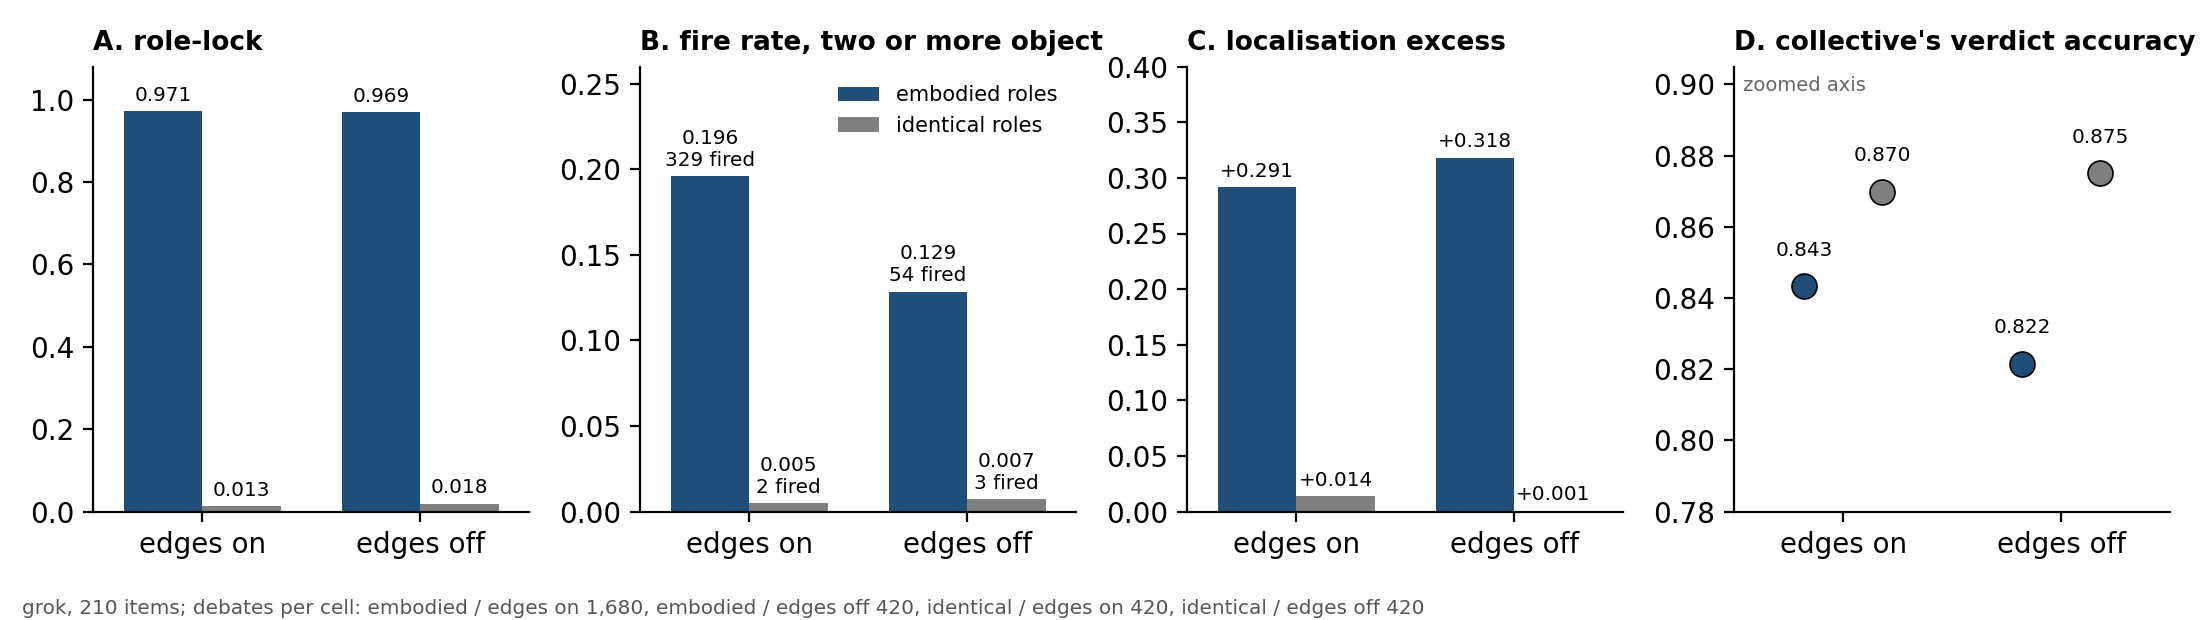
\includegraphics[width=\linewidth]{figures/fig6.png}
\caption{The roles by edges two-by-two on grok. Role-lock, the fire rate of
the counter, the localisation excess and the collective's verdict accuracy
per cell. The structure follows the roles and survives the removal of every
exchange. The identical-reader cells produce none of it and are the most
accurate.}
\label{fig-topology}
% make_figures.py Fig 6, regenerated 2026-09-12 from topology_2x2_analysis.json cells.*
% (role_lock 0.971/0.969/0.013/0.018; fire 0.196/0.129/0.005/0.007 with n_fired 329/54/2/3;
% localisation_excess +0.291/+0.318/+0.014/+0.001; s2_acc 0.843/0.822/0.870/0.875), prereg 16.10 RESULTS
\end{figure}

\begin{figure}[t]
\centering
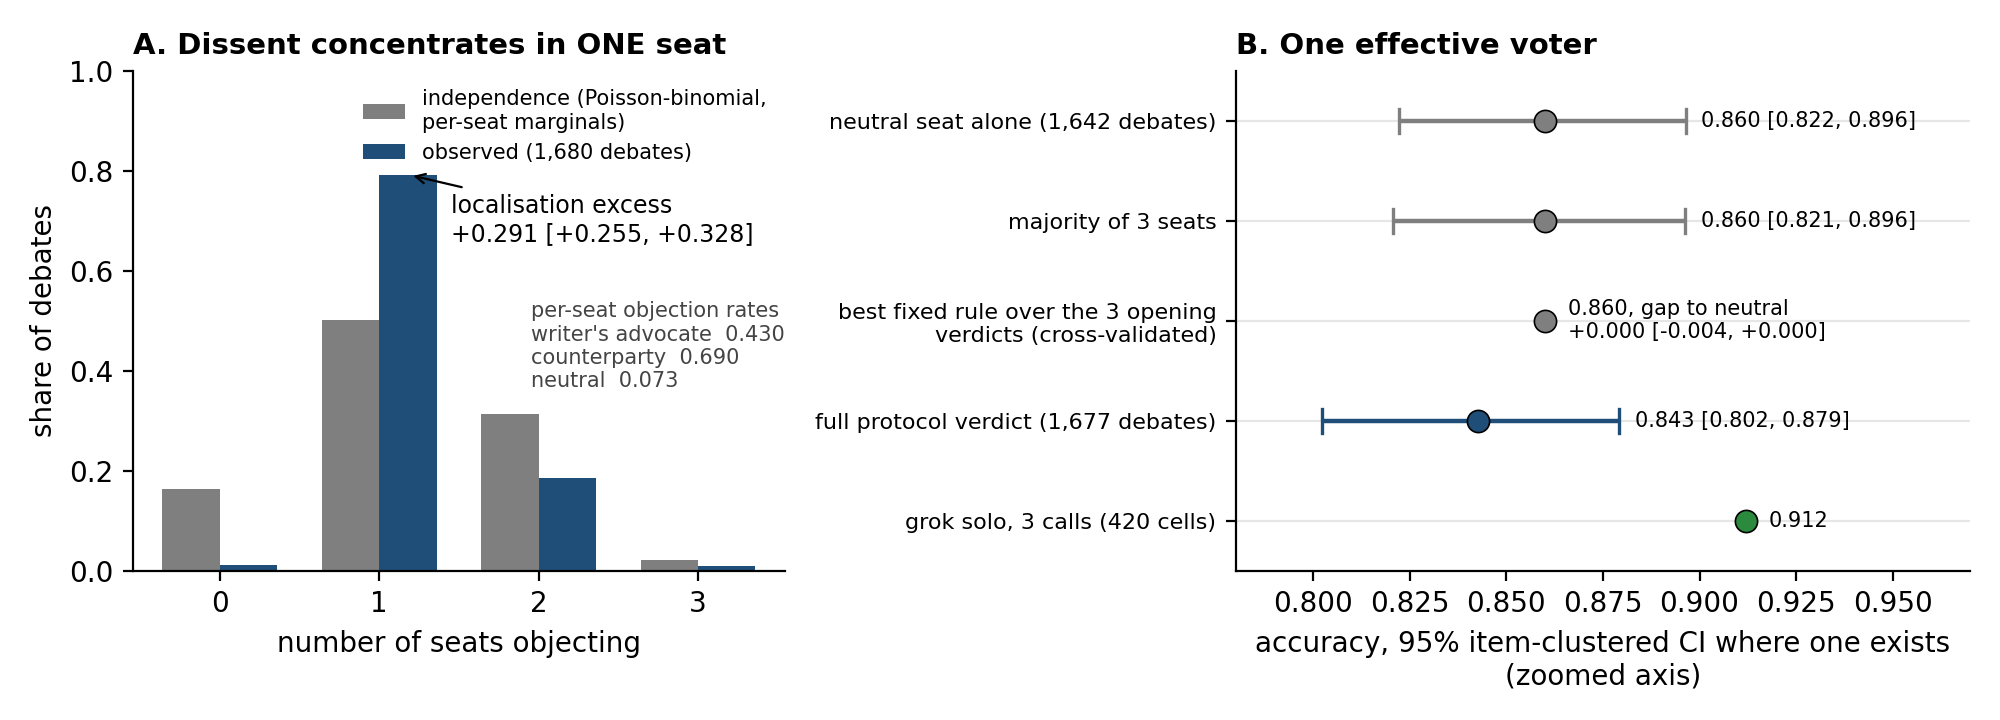
\includegraphics[width=\linewidth]{figures/fig4.png}
\caption{Structure of the dissent and the effective voter count on grok.
(A) Number of seats objecting, observed against a Poisson-binomial null from
the per-seat marginals. (B) Accuracy of the neutral seat, the three-seat
majority and the cross-validated oracle over the three opening verdicts on
the 1,642 debates with three codable opening verdicts, the full protocol's
verdict on 1,677 codable debates, and grok alone at majority-of-three on 420
cells.}
% make_figures.py Fig 4, regenerated 2026-09-12. Panel A from
% unembodied_ablation_analysis.json localisation.observed / independence_poisson_binomial
% (prereg L3402, 16.8 RESULTS). Panel B from effective_voter.json panels.grok
% seat_acc_on_triples.neutral_adjudicator 0.860, majority_acc_on_triples 0.860,
% cv_oracle_bits.cv_oracle_acc 0.860 (prereg L4462-4475, 16.15.4 RESULTS);
% router_decomposition.json composed_haiku.routers.collective_alone.composed.acc 0.843
% (prereg L4287); transfer_readouts.json targets.grok_solo_standard.solo_accuracy 0.912
% (prereg L4381-4382). The former phi panel is dropped for budget; the phis are now
% carried by flooding_analysis.json under prereg L4992-5016 (16.12 RESULTS note), see
% header note (f), and can be restored via make_figures.py.
\label{fig-localisation}
\end{figure}

\subsection{The dissent is an error sensor on one-loser verdicts}
\label{sec-results-sensor}

A one-loser verdict undermines exactly one advocate, so on grok exactly one
seat objected
on 0.792 of debates against 0.501 under an independence null from the
seats' own objection marginals, a localisation excess of +0.291
[+0.255, +0.328] (Figure~\ref{fig-localisation}A).
% unembodied_ablation_analysis.json:148-174,181-185 baseline_full_panel (0.7923 vs 0.5008,
% marginals 0.430 / 0.690 / 0.073, excess 0.2914 [0.2545, 0.3283]). The excess survived the
% stake-free control, +0.266 [+0.221, +0.310] against +0.280 [+0.241, +0.317] on 194 items,
% prereg L3402, L3408 (16.8 RESULTS), dropped from the prose for budget.
The registered composite flag fired on 337 of 1,677 codable debates,
lifting the probability of a wrong synthesis by +0.325 [+0.236, +0.416],
% prereg L582, L594-595, L601 (L1 RESULTS; precision 0.409, recall 0.550); definition
% analyze_loop_step.py:109-111; integrated verdict 0.092 -> 0.418,
% claim_audit_analysis.json:97-117 (check2_decomposition)
and the stake-blind counter, two or more seats objecting, fired on 328,
% prereg L4277 (16.15.1 RESULTS pooled row, 328 of 1,677) and L4293 (counter router, 328
% routed); router_decomposition.json counter_lift_by_stratum.pooled.n_fired 328,
% claim_audit_analysis.json:9-10 (n_objectors_ge2 n_fire 328). The nesting of the 328
% inside the 337 (prereg L3071-3075, Addendum 16.1) sits under a non-RESULTS heading with
% no artefact field for the intersection and is not claimed.
with integrated-verdict error rates of 0.415 against 0.095, +0.320
[+0.239, +0.404], a ratio of 4.37, % prereg L4277 (16.15.1 RESULTS pooled row, 328 of 1,677); router_decomposition.json counter_lift_by_stratum.pooled
the composite's advantage as a router being +0.001 [+0.000, +0.003], so
the introduction's sensor is this counter.
% claim_audit_analysis.json:12-16 (composite_minus_rival_natural 0.0012 [0.0, 0.0030])

The pooled ratio mixes two signals. Of the 328 firings, 93 sat on the 1,287
one-loser verdicts and 235 on the 390 both-party verdicts. Within one-loser
verdicts the collective was wrong on 0.387 of flagged debates against 0.039
of unflagged, +0.348 [+0.201, +0.493], a ratio of 9.83, and within
both-party verdicts on 0.426 against 0.523, -0.097 [-0.233, +0.043].
% prereg L4263-4276, L4352-4356 (16.15.1 RESULTS); router_decomposition.json
% stratum_counts, counter_lift_by_stratum.one_loser (0.3871 / 0.0394, 0.3477
% [0.2007, 0.4930], ratio 9.834) and .both_party (0.4255 / 0.5226, -0.0970 [-0.2332, +0.0430])
The dissent is the signal where the verdict has one loser and the verdict
type where it does not. As a router to the haiku judge the
verdict type alone composed at 0.894 against the counter's 0.880, +0.014
[-0.003, +0.030], and their union at 0.905, +0.011 [-0.001, +0.024] over
the verdict type.
% prereg L4291-4303 (16.15.1 RESULTS); router_decomposition.json composed_haiku.routers.*.composed
% (0.894 [0.860, 0.924], 0.880 [0.844, 0.913], 0.905 [0.870, 0.935], intervals dropped from the
% prose for budget), paired_deltas.verdict_type_minus_counter, union_minus_verdict_type
With the cached sonnet judge the three routers composed at 0.913, 0.936 and
0.956 and the union's gain over the verdict type, +0.021 [+0.011, +0.033],
excluded zero. % prereg L4315-4325, L4370-4376; router_decomposition.json composed_sonnet.block
Whether the two add depends on the judge. Grip, the registered
precondition, held on grok alone among four models (Table~\ref{tab-sensor}).
% stake_grip_analysis.json grok-4-1-fast-reasoning:cg_deliberation (G3 0.6309 [0.5865, 0.6728]),
% claude-haiku-4-5:cg_deliberation_haiku_fixed (0.0625 [0.0160, 0.1077]),
% gpt-5.4-nano:cg_deliberation_nano (0.0338 [0.0182, 0.0505]),
% claude-sonnet-4-6:cg_deliberation_sonnet_fixed (0, G2 0.000); definition prereg L1169-1179;
% the four G3 values and intervals are in Table tab-sensor.

The counter also concentrated the errors of generators that never saw the
debate, on three of four readouts (Table~\ref{tab-sensor},
Figure~\ref{fig-transfer}). On the 420 cells, grok answering alone at
0.912 was wrong 4.40 times as often where the counter flagged,
+0.212 [+0.085, +0.359], % prereg L4435, L4440-4441 (16.15.3 RESULTS, counter column; 0.275 vs 0.062 on 420 cells); transfer_readouts.json targets.grok_solo_standard.by_sensor.counter, solo_accuracy 0.9119
and over the 1,287 and 390 debates that transfer lived in the one-loser
stratum, +0.130 [+0.026, +0.258] against +0.017 [-0.087, +0.122].
% prereg L4328-4340 (16.15.1 RESULTS, transfer within strata, debate population with each
% cell's solo verdict replicated over its debates); router_decomposition.json transfer_within_strata
Nano gave +0.216 [+0.064, +0.383] on 407 codable cells and haiku +0.119
[-0.010, +0.271], so with both grok readouts within-model, one of two
cross-vendor readouts excludes zero, which is the claim's scope.
% prereg L4436-4442, L4452-4458 (16.15.3 RESULTS, counter column and pre-declared reading);
% transfer_readouts.json targets.nano_standard (n 407, 13 tie cells dropped) / haiku_standard
% .by_sensor.counter, n_targets_ci_excludes_zero_counter 3; grok narrated +0.282
% [+0.143, +0.435] in Table tab-sensor
The solo model's own free signals did as much, any both-party verdict
among its three samples concentrating its errors 8.20 times and
disagreement among them 6.35, against the counter's 4.40, each composing
with the same judge within 0.005 of the counter's 0.914, no pairwise
difference excluding zero.
% prereg L4386-4399, L4412-4423 (16.15.2 RESULTS, demotion triggers); router_decomposition.json
% solo_signals.signals.any_eshnah (lift +0.243 [+0.131, +0.358], composed 0.919) / disagree
% (+0.332 [+0.163, +0.493], 0.917) / counter (+0.212 [+0.085, +0.359], 0.914),
% paired_vs_counter_natural (+0.005 [-0.012, +0.021], +0.002 [-0.014, +0.019])
By the registered rule the transfer claim is that the collective's flag
concentrates a solo model's errors, and so do its own signals.
% prereg L4412-4423 (16.15.2 pre-declared reading, quoted; the practical claim for other
% generators rests on 16.15.3); router_decomposition.json solo_signals has no union of
% any_eshnah or disagree with the counter, so whether the counter adds to the solo's own
% signals was not measured, and paired_vs_counter_natural includes zero. "So for its own
% errors the solo model needs no collective" dropped for budget; the sonnet paragraph
% below states the missing comparison.

\begin{table}[t]
\centering
\caption{The sensor by model, and its transfer. Top block, each model's own
collective on the crowd panel, with G1 the composite-flag fire rate, G2 the
share of final votes that reject, G3 the stake concentration and $S_2$ the
collective's accuracy. Bottom block, the grok collective's counter applied
to solo generators that never saw the debate, on the codable cells of 420
over 210 items, with the error rate on flagged against unflagged cells, the
ratio and the lift.}
\label{tab-sensor}
\footnotesize
\setlength{\tabcolsep}{2.5pt}
\begin{tabular}{lrcccc}
\toprule
model of the collective & debates & G1 & G2 & G3 & $S_2$ acc. \\
\midrule
grok   & 1,677 & 0.201 & 0.333 & +0.631 [+0.587, +0.673] & 0.843 \\ % stake_grip_analysis.json grok-4-1-fast-reasoning:cg_deliberation (G1 0.2010, G2 0.3333, G3 0.6309 [0.5865, 0.6728], s2 0.8426); prereg L1307
haiku  & 192   & 0.458 & 0.069 & +0.062 [+0.016, +0.108] & 0.885 \\ % stake_grip_analysis.json claude-haiku-4-5:cg_deliberation_haiku_fixed (0.4583, 0.0694, 0.0625 [0.0160, 0.1077], 0.8854); prereg L1308
nano   & 828   & 0.854 & 0.024 & +0.034 [+0.018, +0.051] & 0.829 \\ % stake_grip_analysis.json gpt-5.4-nano:cg_deliberation_nano (0.8539, 0.0242, 0.0338 [0.0182, 0.0505], 0.8285); prereg L1309
sonnet & 31    & 0.065 & 0.000 & 0 (no rejects)          & 1.000 \\ % stake_grip_analysis.json claude-sonnet-4-6:cg_deliberation_sonnet_fixed (0.0645, 0.0, 0.0, 1.0); prereg L1310
\midrule
solo generator & cells & \multicolumn{2}{c}{wrong, flagged vs not} & ratio & lift \\
\midrule
grok, standard & 420 & \multicolumn{2}{c}{0.275 vs 0.062} & 4.40 & +0.212 [+0.085, +0.359] \\ % transfer_readouts.json targets.grok_solo_standard.by_sensor.counter; prereg L4435
grok, narrated & 420 & \multicolumn{2}{c}{0.353 vs 0.070} & 5.01 & +0.282 [+0.143, +0.435] \\ % transfer_readouts.json targets.grok_solo_narrative.by_sensor.counter; prereg L4436
nano           & 407 & \multicolumn{2}{c}{0.375 vs 0.159} & 2.36 & +0.216 [+0.064, +0.383] \\ % transfer_readouts.json targets.nano_standard.by_sensor.counter (13 tie cells dropped); prereg L4437
haiku          & 420 & \multicolumn{2}{c}{0.255 vs 0.136} & 1.88 & +0.119 [-0.010, +0.271] \\ % transfer_readouts.json targets.haiku_standard.by_sensor.counter (includes 0); prereg L4438
\bottomrule
\end{tabular}
\end{table}

\begin{figure}[t]
\centering
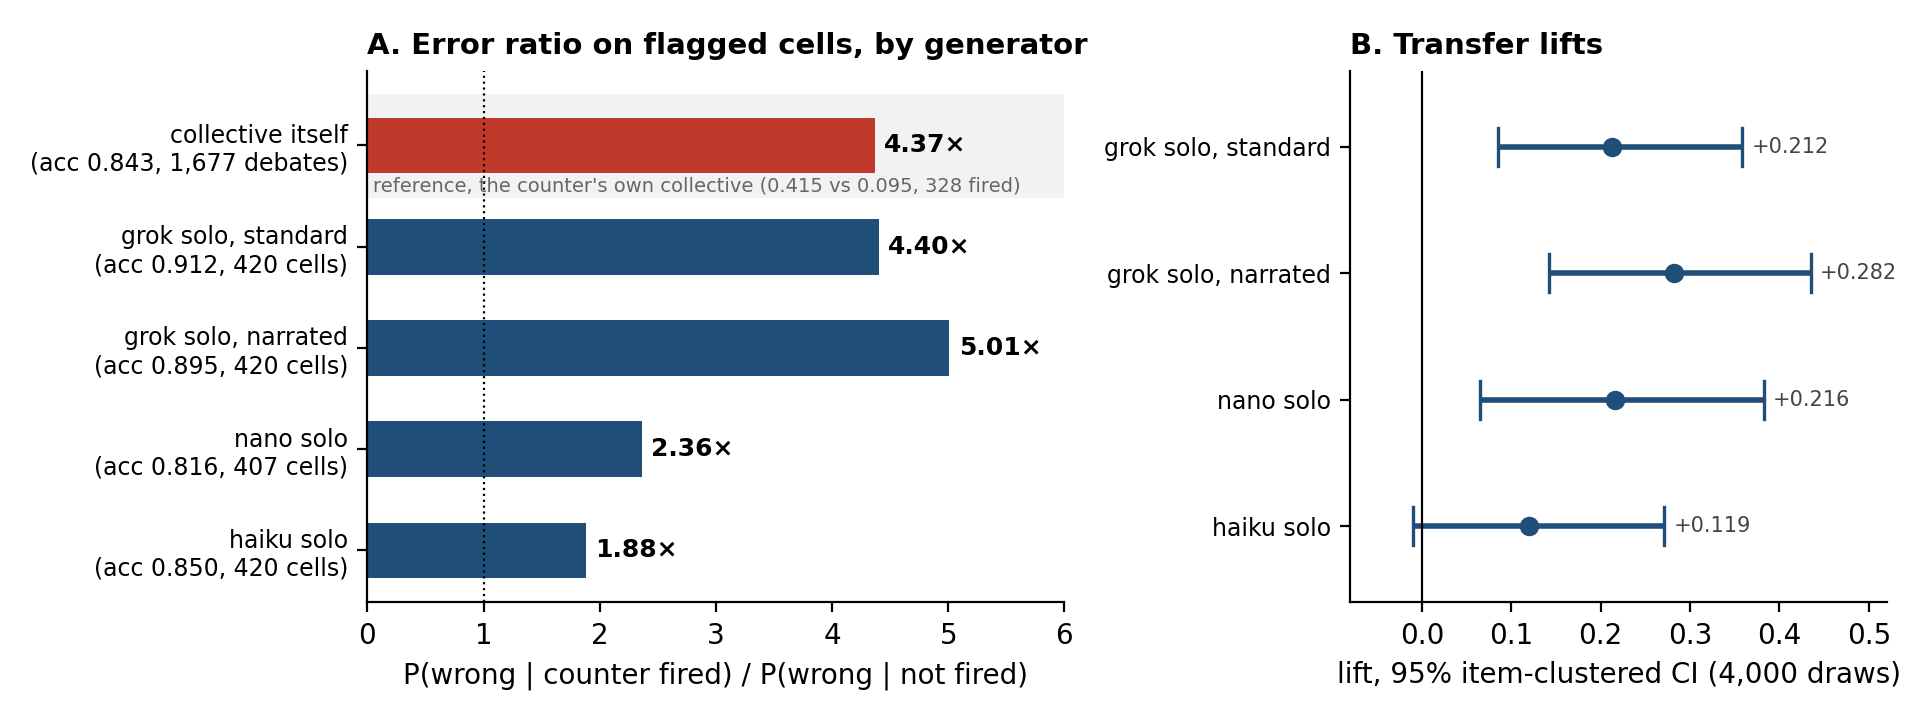
\includegraphics[width=\linewidth]{figures/fig3.png}
\caption{Transfer of the counter. (A) Ratio of the error rate on flagged to
unflagged cells of item and framing, and debates for the collective, for the
collective itself and for four solo generators the flag never touched. (B) Item-clustered intervals and point estimates on the
four transfer lifts.}
% make_figures.py Fig 3, regenerated 2026-09-12 from transfer_readouts.json
% targets.*.by_sensor.counter (ratios 4.40 / 5.01 / 2.36 / 1.88, lifts and CIs as in
% Table tab-sensor, solo accuracies from targets.*.solo_accuracy) and
% router_decomposition.json counter_lift_by_stratum.pooled (4.37, 0.415 vs 0.095) for the
% collective; prereg L4277 (16.15.1) and L4435-4438 (16.15.3). A point estimate is drawn
% on every row.
\label{fig-transfer}
\end{figure}

Routing on the flag paid over the collective (Figure~\ref{fig-routing}).
The haiku judge on the 337 flagged debates raised their accuracy from 0.582
to 0.774, +0.193 [+0.067, +0.310] at the Bonferroni-corrected 98.75 percent
level, and on the unflagged debates moved it -0.040 [-0.100, +0.016], so
at 95 percent the composed system at 0.881 beat the collective by +0.039
[+0.018, +0.060] and the judge used everywhere, 0.850, by +0.032
[-0.004, +0.068], a gain the record does not claim.
% prereg L856, L858, L866-867 (98.75 percent family; the -0.040 shares the level of the
% +0.193, L859 header "delta [98.75% CI]"), L885-886 and L889-895 (composed system, "95%
% item-clustered CIs"; "beats haiku alone directionally (the second interval touches zero;
% not claimed as established)"); actuator_ladder_analysis.json A3a and A3a_unflagged
% (ci_level 0.9875, lo 0.0667 hi 0.3099; lo -0.0997 hi 0.0162). The composed 0.881 is the
% composite router; the counter's 0.880 [0.844, 0.913], +0.038 [+0.016, +0.060], is in
% router_decomposition.json composed_haiku (point given above, interval in its comment).
A stronger judge met the first registered criterion and not the second.
% prereg L3593 (registration, positive iff routed beats BOTH grok-solo and sonnet-everywhere), L3624-3626 (16.11a RESULTS)
Routing grok's solo verdicts to sonnet on the counter raised 0.912 to
0.936, +0.024 [+0.005, +0.045], on the same 420 cells where the composite
flag gives the same result, and sonnet on every cell scored 0.976, so
routing on the flag sits 0.041 [0.014, 0.069] below the judge used
everywhere. % prereg 16.22 RESULTS (routing_certification.json: sonnet judge, counter 51 fired, coverage 0.121, routed 0.9357, delta over base +0.0238 [+0.0048, +0.0452]; composite +0.0238 identical; vs sonnet everywhere -0.0405 [-0.0690, -0.0143]); the 16.11a composite figures reproduce exactly on the 418-cell population (0.9354, +0.0239)
The same cells routed on the solo model's own three-sample disagreement
reached 0.938, +0.026 [+0.010, +0.045], not distinguishable from the
counter, +0.002 [-0.019, +0.024], at three calls per case against
seventeen, and routing on any both-party verdict among the solo's samples
reached 0.960. % prereg 16.22 RESULTS (disagreement -> sonnet 0.9381, +0.0262 [+0.0095, +0.0452]; disagreement minus counter +0.0024 [-0.0190, +0.0238]; any ESH/NAH -> sonnet 0.9595, +0.0476 [+0.0190, +0.0786]; reading R3)
Priced from the cached token counts, the solo model alone costs
\$0.0005 a case, the solo routed on its own disagreement \$0.0014, the
collective's sensor routed to the same judge \$0.0098, and the judge
everywhere \$0.0115, so for a solo model's errors the collective's flag
is dominated on cost by the model's own disagreement, and its value is as
an audit of the collective's own verdicts and as the structure in which
the information sits. % prereg 16.22 RESULTS (cost_per_decision: base 0.912 at $0.00049, disagreement -> sonnet 0.938 at $0.0014, counter (k=1, 17 calls) -> sonnet 0.936 at $0.0098, sonnet everywhere 0.976 at $0.0115; reading R5); PI instruction 2026-09-14, no stronger case than the record justifies

\begin{figure}[t]
\centering
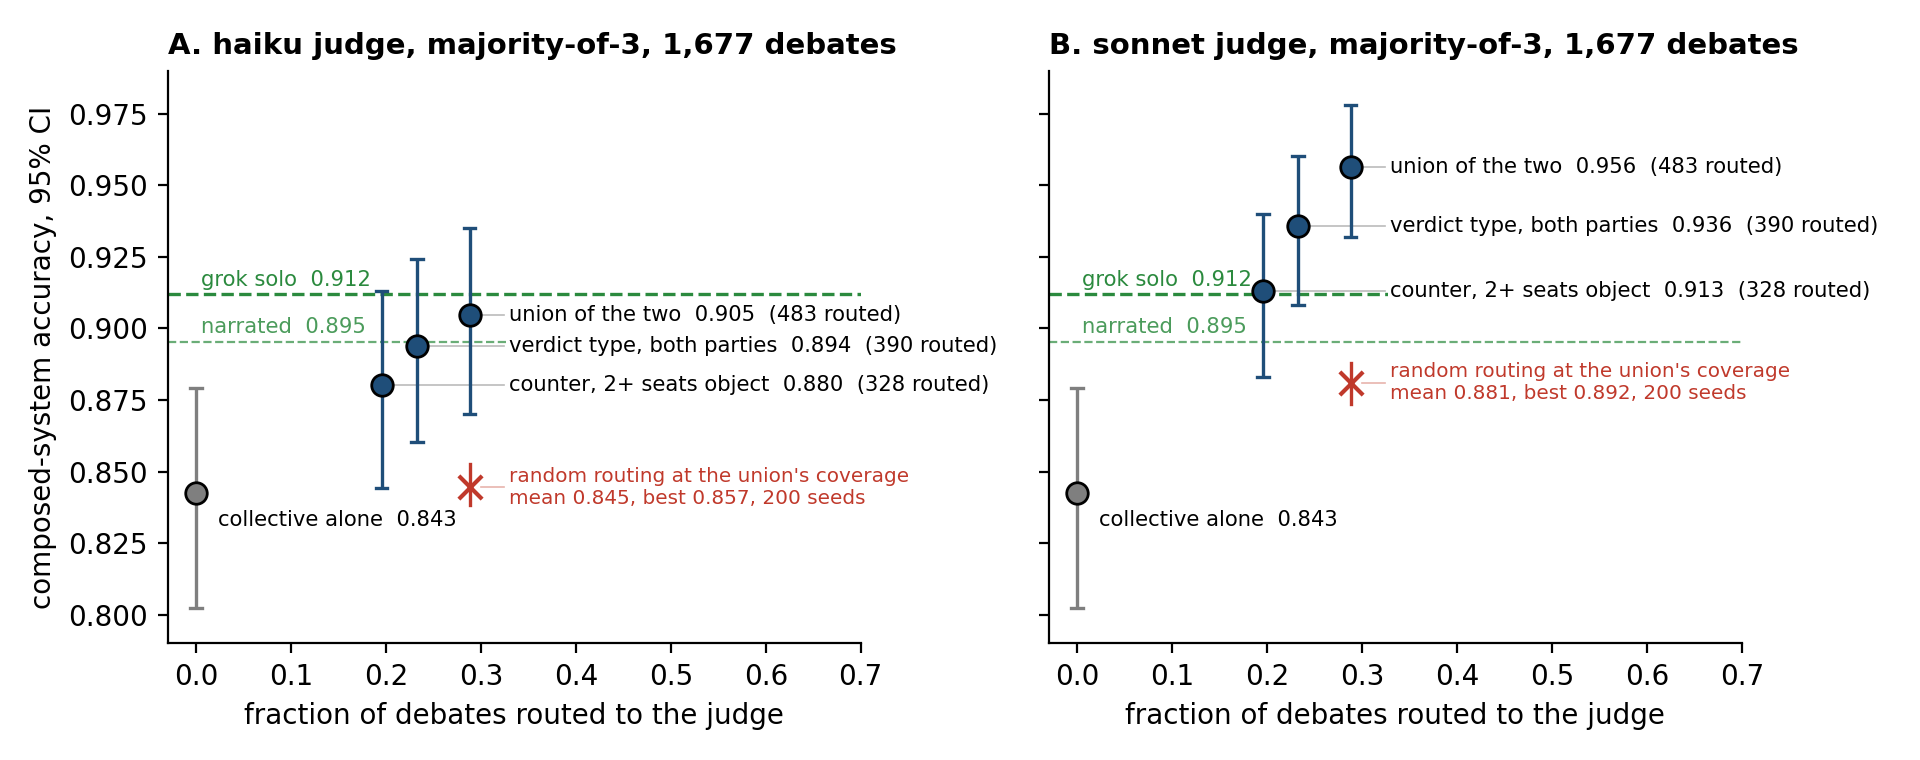
\includegraphics[width=\linewidth]{figures/fig5.png}
\caption{Composed-system accuracy against the fraction of debates routed to
the judge, for the counter, the verdict-type router and their union, with
random routing at the union's coverage and the two solo grok baselines
marked. Panel A routes to the haiku judge and panel B to the sonnet judge
of the second design.}
% make_figures.py Fig 5, regenerated 2026-09-12 from router_decomposition.json
% composed_haiku.routers (collective_alone 0.843 at 0, counter 0.880 at 0.196, verdict_type
% 0.894 at 0.233, union 0.905 at 0.288) and random_at_union_coverage (mean 0.845, best
% 0.857, 200 seeds) and composed_sonnet.routers (0.843 / 0.913 / 0.936 / 0.956, random
% mean 0.881 best 0.892), prereg 16.15.1 RESULTS; solo baselines
% transfer_readouts.json targets.grok_solo_standard / grok_solo_narrative.solo_accuracy
% (0.912 / 0.895). The former html-only points (both sensors fire, own samples disagree,
% html union) are gone.
\label{fig-routing}
\end{figure}

\subsection{Who decides changes the verdict, and who is seated changes it too}
\label{sec-results-decider}

Four ablations vary the graph itself, holding the two locked advocates and
their account fixed, to ask what the moderator and the seating do to the
verdict and to the sensor separately.

Replacing the grok moderator with sonnet over byte-identical, locked seats
raises the collective's verdict accuracy from 0.848 to 0.885,
$+0.038$ $[+0.014, +0.064]$; replacing it with haiku instead lowers accuracy
to 0.735, $-0.115$ $[-0.169, -0.060]$, below haiku answering the same items
alone (0.851).
% 16.17 RESULTS cells 1 and 2; cg_deliberation_modsonnet_analysis.json,
% cg_deliberation_modhaiku_analysis.json
The seats' own behaviour does not move with the moderator. Role-lock is
identical by construction (the opening statements are replayed), and
localisation excess (+0.300 sonnet, +0.239 haiku, against +0.291 pooled) and
the counter's fire rate stay within the range the moderator-free cells
already show. What moves is the verdict itself and, through it, which
verdicts the sensor sees. The haiku moderator issues an everyone-or-no-one
verdict on more than a quarter of debates (0.300 against 0.243 for grok and
0.176 for sonnet), which floods the counter and collapses its pooled lift
to $+0.070$ $[-0.026, +0.170]$; the within-one-loser lift, which the
flooding does not touch, is the reading that survives. The moderator is
therefore not a neutral aggregator of what the seats already decided. It is
the node whose own competence sets the verdict and whose own habits about
naming everyone at fault set how often the sensor is even asked to speak,
while the seats' structure is invariant to it.

Replacing the three seats themselves with three uninterested readers from
three vendors (haiku, nano, grok, no assigned side) tests whether the
same-model bottleneck of Section~\ref{sec-results-collective} is a same-model
problem or a same-opinion problem. Errors across vendors are far less
correlated than errors across samples of one model (mean pairwise phi
$+0.253$ against $+0.65$ pooled), and the majority does approach the
independence prediction, but the panel's weakest reader (haiku, 0.697) is
weak enough that the majority still does not clear its best member at the
opening statement, $+0.011$ $[-0.013, +0.034]$, and after one further round
it does, $+0.031$ $[+0.005, +0.057]$, the one cell in the programme where a
three-seat majority beats its best single seat with an interval excluding
zero.
% 16.18 RESULTS; multivendor_analysis.json
Neither reading changes the standing result: the cross-vendor panel is not
more accurate than three grok readers ($-0.010$ $[-0.033, +0.013]$ on the
collective's verdict) and not a better answerer than the best model alone
($-0.055$ $[-0.087, -0.024]$). The panel does produce an objection
structure with no assigned stake at all (fire 0.401, lift $+0.121$
$[+0.044, +0.201]$), disagreement among unequal readers rather than dissent
against interest, and it is weaker on every readout than the embodied
sensor. Composed as a router ahead of a stronger judge it beats the
collective alone ($+0.024$ $[+0.009, +0.042]$) but not a single cheap
judge call of a stronger model, so a decider panel across vendors buys
nothing a moderator selected for competence does not already buy.

Adding a second, like-biased advocate to the writer's side (four seats: two
for the writer, one for the counterparty, one uninterested) tests whether
the sensor is about sides or about seats. The second writer-side seat
copies its principal's opening verdict on 99.5 percent of debates and its
objections at $\phi=+0.975$ $[+0.952, +0.995]$, and adds no lift to any
reconstruction of the counter once the extra seat is accounted for
(pooled two-of-four lift $+0.294$ $[+0.206, +0.383]$ against the three-seat
reconstruction's $+0.324$ $[+0.224, +0.422]$, a difference of $-0.030$
$[-0.111, +0.053]$).
% 16.19 RESULTS; coalition_analysis.json
The sensor scales with distinct sides, not with seats. The verdict does
not: with two seats on one side the collective's accuracy falls by
$-0.074$ $[-0.117, -0.031]$ and its at-fault rate falls by $-0.121$
$[-0.154, -0.088]$, concentrated on the items where the writer is at fault
(0.808 to 0.570 on gold-guilty items). An unequal graph manufactures bias
at the decider even when every advocate is individually locked to its
assigned side, which is the one finding in this batch that bears directly
on deployment: representation in the graph is itself a lever on the
verdict.

Extending the graph to a third party named in the account but not seated
in the original three (accounts where the writer's story implicates
someone else's decision) tests the credible-signal principle's scope
directly. The writer and counterparty stay locked (0.959); the added
third-party advocate does not, arguing its assigned stake only 0.800 of
the time, and its own against-interest objection rate lands well above
the 0.10 the two-party principle predicts (0.198, against the writer's
0.081). With three advocates a verdict undermines exactly one of them on
241 debates and two of them on 72; the against-interest count still works
within the one-undermined case ($+0.162$ $[+0.051, +0.289]$, 69 fired,
transfer to grok solo $+0.078$ $[+0.001, +0.160]$) and a plain two-or-more
counter floods once two advocates are undermined together, exactly as
predicted (fire 0.353 to 0.861).
% 16.21 RESULTS; nperspective_analysis.json
What fails is the one-dimensional reading of the stake: at two-undermined
debates the co-losers object together only 0.695 of the time, not near
certainty, because a two-party verdict token does not encode every
dimension along which a third party's interest can be undermined. The
sensor degrades gracefully where the graph grows along a new axis; the
verdict again pays a cost for the extra seat ($-0.045$ $[-0.087, -0.006]$
against the three-seat cell on the same debates), the same direction 16.19
found.

\subsection{The extent of the method}
\label{sec-results-extent}

The sensor reads departures from role, so it fails in three measured ways. On
the paired-account corpus, where the verdict names which of two actions was
worse, grip was the strongest we measured, +0.670 [+0.627, +0.710] on
624 codable debates. % prereg L2598-2599 (Stage 2 RESULTS; reject 0.772 undermined vs 0.102 not, L2600-2601); Stage 1's +0.755 [+0.659, +0.848] on 75 codable debates, prereg L2428-2429, dropped for budget
The advocates tracked their interests so well that the composite flag fired
on 6 of 624 debates and both advocates rejected on none, % prereg L2594; L2732 (13.1 RESULTS table, both_advocates_reject 0 of 624, the counter's own silence)
and a registered search over eleven native dissent statistics promoted
none. % prereg L2700-2703, L2735-2736 (13.1 RESULTS); dilemma_sensor_search_analysis.json
The sensor went silent.
% The haiku judge on those six moved accuracy 0.667 -> 0.500, -0.167 [-0.500, +0.000] at
% 97.5 percent, prereg L2613; dilemma_stage2_actuator_analysis.json:5-14. Dropped for budget.
% The flag's apparent lift on the raw population, +0.314, was an abstention artefact (16
% of 22 raw-flagged debates non-codable; -0.023 on the codable population),
% claim_audit_analysis.json check3_dilemma, prereg L3118-3122, dropped from the prose.

Where the verdict finds everyone at fault or no one, both advocates lose and
the sensor floods, firing on 0.603 of grok's 390 both-party verdicts
against 0.072 of its 1,287 one-loser verdicts, so there the verdict type
is the error signal, not the dissent (Section~\ref{sec-results-sensor}).
% prereg L4266-4268, L4273-4276 (16.15.1 RESULTS, strata 1,287 / 390, fired 93 / 235),
% L4358-4368 (the both-party lift -0.097 [-0.233, +0.043] is given in sec-results-sensor);
% router_decomposition.json stratum_counts, counter_lift_by_stratum.one_loser.coverage
% 0.0723 and .both_party.coverage 0.6026, composed_haiku.routers.collective_alone
% .by_stratum.acc_s2 0.9355 and 0.5359 (the collective wrong on 0.464 of both-party against
% 0.064 of one-loser verdicts, dropped from the prose for budget). The Addendum 16.12 table
% (L3666-3668) is reproduced under a RESULTS heading at prereg L4992-5016 with
% flooding_analysis.json (its 1,288 / 0.922 / 0.614 / 0.576 on the S2-codable population
% and the per-type phis, header note (f)); the prose keeps the 16.15.1 population.

Without a real counterparty the roles moved the vote little. On the
false-premise problems a majority-of-three panel mixing author, neutral and
rival affirmed the false premise at 0.162 against 0.188 for three
authors, -0.026 [-0.047, -0.007], and -0.010 [-0.031, +0.008] against
three disinterested judges.
% prereg L4569-4571, L4574-4575 (16.15.6 RESULTS); bm_notes.json 16.15.6 plain.panels, plain.deltas;
% also prereg L172-178 (E1 RESULTS); the panel intervals 0.162 [0.103, 0.226] and 0.188
% [0.125, 0.257] (L4569-4570) dropped for budget
It rejected the premise no more often, -0.001 [-0.025, +0.022], and
abstained more, +0.027 [+0.000, +0.054], so it lowered false affirmation
by abstaining more, not by rejecting more, no gain in accuracy under the
rule that non-commitment is never correct.
% prereg L4569-4571, L4586-4591 (16.15.6 RESULTS, the required wording; P(FALSE) 0.552
% against 0.552, P(abstain) 0.286 against 0.260, rates dropped for budget); bm_notes.json
% 16.15.6 snapshot_plain.panels.*.p_false / p_abstain and deltas
Under narration the same contrast fell to -0.004 [-0.025, +0.016] and the
mixed panel itself rose by +0.044 [+0.012, +0.079], so narration's error
passed through the vote. % prereg L369-374 (E2 RESULTS), L4576-4580; bm_cross_sig_analysis.json:97-108
% The gpt-4o screen that failed the registered guard (prereg L3641-3646, 16.11b RESULTS; a
% platform content filter emptied 15 percent of integration calls; the G3 it printed must
% not be tabulated) is stated in methods.tex sec-method-estimation and dropped here for budget.

The same theory marks a joint-action frontier, and every regime of its
instrument fell outside the theory's domain for a measured reason. On 144
ordinal two-by-two games under a binding joint plan, grok alone scored
0.891 [0.840, 0.935] and 48 of 48 in the value region, against the 0.215
floor with payoffs masked.
% prereg L4721-4733 (16.13 RESULTS, Stage A); game_solo_analysis.json overall.accuracy
% 0.8912 [0.8403, 0.9352], by_region.value.accuracy 1.0 (n 48); game_solo_masked_analysis.json
% overall.accuracy 0.2153, verdict_counts NO_UNIQUE_PLAN 432
Seated for the two players the advocates barely locked, 0.094
[+0.031, +0.167] beside a neutral seat and 0.115 [+0.042, +0.198] beside a
mediator, neither ever named the mutual-private cell, both collectives
scored 48 of 48 and no seat objected, so the sensor was silent, not
flooded.
% prereg L4735-4767 (16.13 RESULTS, Stage B1 table and mechanical readings: P1 FAILS, P2
% FAILS, P3 NULL at a ceiling, P5 not observed, "SILENT here, not flooded");
% game_B1_analysis.json arms.*.role_lock.all.signed (0.0938 [0.0313, 0.1667] neutral,
% 0.1146 [0.0417, 0.1979] planner), nash_pull.per_seat.*.r0.by_gold_type
% .DILEMMA_BOTH_PREFER 0.0 both advocates both arms, accuracy.group.final 1.0 (48 of 48)
% both arms, grip.G1_fire_rate 0.0 and per_seat.*.objected_r3 0.0, contrast.stats
% .group_accuracy delta 0.0 [0.0, 0.0] on 16 shared items (the mediator's +0.000
% [+0.000, +0.000] over 16 items, prereg L4755, dropped from the prose for budget).
A plan both must accept removes the conflict the roles need. Over all
144 games the advocates locked at the opening statement, 0.405
[+0.335, +0.474] and 0.385 [+0.322, +0.449], then conceded by the second
round, so the flag never fired on 288 cells, and the one gain over grok
alone was restraint. Where no unique
plan exists the solo model named one on 47 percent of cells, and the
mediator collective declined more often, +0.151 [+0.043, +0.280] over 31
games, against the registered expectation that neither arm would beat the
solo there, while the naive collective's +0.086 [-0.032, +0.226] did not
clear zero.
% prereg L5018-5058 (16.13 RESULTS, Stage B2). Role-lock: L5025 table row "role-lock
% (favours own player), all" 0.405 [+0.335, +0.474] neutral arm, 0.385 [+0.322, +0.449]
% planner arm, computed over all 144 games; game_B2_analysis.json arms[cg_game_neutral_b2]
% .role_lock.all.signed (0.4049 [0.3347, 0.4737], n_debates 144) and arms[cg_game_planner_b2]
% .role_lock.all.signed (0.3846 [0.3217, 0.4491], n 144); by_region value 0.0625 [0.000,
% 0.156] both arms, neutral 0.377 / 0.361, cannot_assist 0.673 / 0.633, and no pooled
% outside-value-region lock exists in the record (L5048-5049 "0.39 to 0.41" is loose), so
% the prose names the population; the in-region 0.094 / 0.115 (prereg L4747, B1 RESULTS)
% are given in the B1 sentence above. "The boundary the paired-account corpus showed"
% (prereg L4778-4781) dropped for budget.
% Concede by r2, L5051-5052; stake-blind flag 0 of 144 per arm, L5031. Solo cannot-assist
% 0.527, "named a plan on 47% of cells that have no unique one", prereg L4729 (16.13
% RESULTS, Stage A). Paired planner - solo cannot-assist +0.151 [+0.043, +0.280] (L5039)
% and neutral - solo +0.086 [-0.032, +0.226] (L5038), 3,000 draws seed 7, "not
% pre-declared beyond P3/P4, reported for the extent map" (L5034-5035), nine contrasts in
% that table with no correction; P4 expected neither arm to beat the solo on cannot-assist
% games (L4025-4028) and is CONTRADICTED for the planner arm (L5041-5046);
% game_B2_analysis.json contrast.
Without enforcement the roles locked completely, the tempted advocate
naming its private action on every opening statement, and so did every
other node, the solo model and the neutral reader recommending the
equilibrium in every dilemma game and the mediator in 20 of 21 cells,
none ever the Pareto cell, so the mediator held nothing, -0.042
[-0.146, +0.042] against the naive reader. In a one-shot dilemma without
enforcement the correlated-equilibrium set is the Nash set, so the
unanimity is the correct answer to the question as put.
% prereg L4961-4990 (16.13c amendment: P1' on tempted seats), L5060-5106 (16.13c RESULTS,
% Stage C1): P1' tempted 1.000 [1.000, 1.000] n 24 both arms (L5066); solo non-binding
% DILEMMA accuracy 0.000, Nash-pull 1.000 (L5075, L5083-5084); third seat r0 Nash-pull in
% DILEMMA neutral_reader 1.000, plan_mediator 0.952 (L5077, L5084-5085), 20 of 21 cells at
% r0 and 1.000 at r2; "No seat, in either arm, ever recommended the Pareto cell"
% (L5085-5086); P3' -0.042 [-0.146, +0.042] FAILS (L5068); the theory's correction
% L5089-5094. game_C1_analysis.json arms[cgnb_game_planner].accuracy.third_nash_pull
% .plan_mediator_nb.r0.by_gold_type.DILEMMA_BOTH_PREFER (n 21, 0.9524 [0.857, 1.0]) and
% .r2 (1.0); arms[cgnb_game_neutral]...neutral_reader_nb.r0 (1.0); game_solo_nb_analysis.json
% by_gold_type.DILEMMA_BOTH_PREFER.nash_pull 1.0, accuracy 0.0.
Where a recommendation can coordinate, in nine games with two equilibria
favouring different players, the solo model declined on every one of 27
rows, which the registration scores as failure because either
equilibrium is self-enforcing once both players hear it, and the
collective coordinated on an equilibrium on 5 and 6 of 27, +0.185
[+0.037, +0.370] over the solo in the neutral arm and +0.222 in the
mediator arm, whose own interval [0.000, 0.481] reaches zero. All eleven
recommendations named an equilibrium, nine the welfare-better one, so
the gain is commitment, not guessing, and the two third seats did not
differ, +0.037 [-0.111, +0.222]. Across every regime the advocates locked
at the opening and yielded by the vote, the opposite of the dispute and
paired-account advocates, so the sensor had nothing to read and a
non-embodied third node steered nothing the naive reader did not, and
whether restraint and coordination owe anything to the opposed advocates
rather than to deliberation itself is not separable here, since the solo
comparator has no third seat and no identical-reader cell was run on the
games.
% prereg L5108-5145 (16.13d registration): L5114-5117 (either equilibrium self-enforcing
% once both hear it, the advocates' interests conflict over which), L5129-5131
% (COORD scoring, "A recommendation of NO_RECOMMENDATION or of a
% non-equilibrium cell counts as failure to coordinate"; D1, D2, D3 readings L5139-5144).
% prereg L5147-5192 (16.13d RESULTS): COORD 0.185 [0.037, 0.333] / 0.222 [0.000, 0.481] /
% solo 0.000 (L5150); NO_RECOMMENDATION share 0.815 / 0.778 / 1.000 (L5152); D2 neutral -
% solo +0.185 [+0.037, +0.370] and planner - solo +0.222 [+0.037, +0.481] (L5159-5160);
% D1 +0.037 [-0.111, +0.222] fails (L5158); WELFARE 4 of 5 and 5 of 6 (L5151, L5167-5169);
% LOCK 0.907 [0.815, 1.000] / 0.870 [0.778, 0.944] (L5153); ACCEPT on the other's
% equilibrium 1.000, n 5 and n 6 (L5155, L5161, D3 yields); flag 0 of 27 (L5156); lock at
% r0 in every regime, conceded by r2, accepted at r4, "The AITA advocates do neither"
% (L5175-5180); the collective beats the solo only where the solo declines, restraint (B2)
% and coordination (D) (L5181-5185); a non-embodied third node steers nothing the naive
% reader does not (L5185-5187). Paired-account advocates hold at the vote: prereg
% L2598-2601 (Stage 2 RESULTS, reject 0.772 undermined against 0.102). Not separable:
% prereg L5054-5057 (16.13 B2 RESULTS, "the solo comparator has no third seat"); every
% games arm carries embodied advocates and the arms differ only in the third seat
% (L4064-4067, L4809, L5119-5121), and the identical-reader cells of 16.10 exist only on
% the disputes (L4136).
% game_coordination_analysis.json arms.neutral.COORD (0.185 [0.037, 0.333]),
% arms.planner.COORD (0.222 [0.000, 0.481], seed 7, scripts/analyze_game_coordination.py:192),
% contrasts "D2 neutral - solo, COORD" (0.185 [0.037, 0.370]) and "D2 planner - solo, COORD"
% (0.222 [0.037, 0.481], seed 18, line 213); solo.COORD 0.000 [0.000, 0.000] and
% NO_RECOMMENDATION_share 1.0, so arm and contrast are one statistic and the planner
% lower bound is a property of the random stream (replayed 2026-09-12 with the analyzer's
% boot over 2,000 draws: 0.000 on seeds 2, 5, 7 and 0.037 on seeds 1, 3, 4, 6, 18; the six
% coordinated planner cells lie in three of nine games, 124, 134, 143, so (6/9)^9 = 0.026 of
% item resamples hold none; the neutral arm's five cells lie in four games, 124, 132, 134,
% 143, and its bound is 0.037 on every seed). arms.*.NO_RECOMMENDATION_share plus
% arms.*.COORD.point equal 1.000 in both arms (0.815 + 0.185, 0.778 + 0.222), so no
% recommendation fell on a non-equilibrium cell (cgnb_game_neutral_d_rows.csv verdicts 22
% NO_RECOMMENDATION, 3 PLAN_11, 2 PLAN_22; cgnb_game_planner_d_rows.csv 21, 2, 2, 1, 1,
% every named plan a Nash cell after permutation); D1 from contrasts.
